\chapter{A Hybrid Method Based on Monte Carlo fragment Sampling \ac{PSPP}}\label{chap:methodology}

This Chapter presents the methods for approaching the \textit{ab initio}
\ac{PSPP}. There are three points that need to be specified for an \textit{ab
initio} method~\cite{dorn2014three}: The protein computational representation,
the energy function and the the conformation sampling procedure. These three
points are visited in
Sections~\ref{sec:computation-representation},~\ref{sec:energy-function}
and~\ref{sec:conformation-sampling}, respectively.

\section{Computational Representation}
\label{sec:computation-representation}

This work aims for a full atom prediction of a given target protein, which
limits the possible representations that can be utilized.  Considering its
properties, a full atom backbone representation was utilized.  The backbone is
manipulated by changing the three dihedral angles $(\phi, \psi, \omega)$.  The
Side chain is abstracted into an ellipsoid of similar mass and shape, in order
to maintain some of its properties. Therefore, the model utilized consists of a
backbone torsion angle representation with side chain ellipsoids.

For this work, the protein model includes more information than just the atoms
and its respective conformation. The model is split into three components and
is illustrated in Figure~\ref{fig:protein-model} using the 1PLW polypeptide as
example. The first component is a pose object that stores the conformation of a
given protein considering all its atoms. This object is responsible for
updating the atoms when an angle is alternated. Such changes must be propagated
down to the chain considering an arm lever effect. The second component of this
model consists of a vector which acts as an interface for the optimization
algorithm and holds all the backbone dihedral angles. The optimizer does not
act directly upon the pose object, instead, it operates on this vector. When
this vector is changed, the pose object changes accordingly. The third
component is another vector containing a sequence of predicted secondary
structures and its confidence intervals. This information is used to coordinate
the sampling procedure.

From Figure~\ref{fig:protein-model}, the top part consists of the pose model,
responsible for holding the atom representation of the protein. The middle part
consists of a vector of dihedral angles. Since 1PLW has 5 amino acids, the
angle vector has 15 elements.  The first three elements represents the $(\phi,
\psi, \omega)$ angles for the first amino acid, the second three elements
represents the dihedral angles for the second amino acid and so on. The bottom
part models the predicted secondary structure. For the 1PLW it consists of
simply a coil along all the protein.  Each cell of this vector holds the
probabilities for each predicted secondary structure.  For instance, the middle
amino acid in 1PLW named GLY could have $(C=0.9123, A=0.0731, B=0.0146)$,
meaning that the predicted probability of that amino acid being a coil is of 91
percent, 7 percent for an $\alpha$-helix and 1 percent for a $\beta$-sheet. In
the actual model all 8 classes presented in
Section~\ref{sec:secondary-structure-prediction} are considered.

\begin{figure}
    \centering
    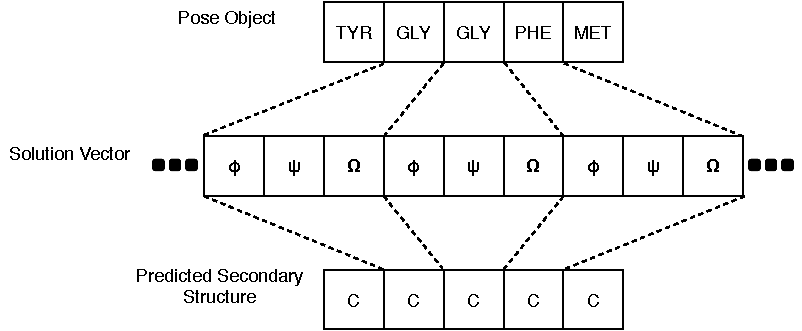
\includegraphics{Figuras/protein-representation.pdf}
    \vspace{1mm}
    \caption{The Protein Computational Model (Source: Author)}
    \label{fig:protein-model}
\end{figure}

The secondary structures are classified using a DSSP8
notation~\cite{frishman1995knowledge}.  For this work they were predicted using
the PSIPRED\footnote{Available for academic use in:
\url{http://bioinf.cs.ucl.ac.uk/psipred/}}  server~\cite{mcguffin2000psipred}. The knowledge from the secondary
structure prediction is incorporated in the model using fragment insertion,
which will be further explained in Section~\ref{sec:conformation-sampling}.

At the end of the prediction, the output consists of a full atom protein
representation, including the side chains. For this, an off-the-shelf repacker
available in Rosetta toolkit was utilized.  The repacker replaces the
ellipsoids with the actual side chains. This introduces a series of (potential)
hysterical clashes between the side chains, specially in more densely packed
structures. To solve this problem, a gradient descent optimization is
performed, where the Van der Waals repulsive forces are slightly varied during
the gradient descent.  With this, the gradient descent can rotate the side
chains and move the backbone in order to make room for the newly inserted side
chain structures.  The final result of this is a full atom representation of
the predicted protein, which is the output of the proposed approach.

\section{Energy Functions Employed}
\label{sec:energy-function}

The energy function represents the domain information from the \ac{PSPP} in a
mathematical equation. Different energy functions considers different aspects
of the problem, which can be useful for different steps of the prediction. This
work makes use of three energy functions available in Rosetta.

The first energy function utilized is referenced in Rosetta as score0. This
energy function consists solely of the repulsive Van der Waals forces. The goal
of this energy is to aid the generation of initial conformations. Since only
the repulsive forces are considered, a score0 with a value of $0$ indicates
that a given conformation has no clashes between different parts of the
protein. The assembly of the protein guided by the score0 function leads to
more plausible starting proteins.

The second energy function utilized is referenced in Rosetta as score3. It uses
a full atom representation of the backbone and an ellipsoid to represent the
side chains. A more in depth explanation of this energy function is explained
in~\cite{alford2017rosetta}. Unfortunately, the only up to date documentation
found for the energy functions is the Rosetta source code itself.  The score3
energy function is used during the main portion of the prediction process
described next section.

Finally, the last energy function is the scorefxn, as found in Rosetta. It
encompasses the same information as score3, however, it considers a full atom
representation of the side chain as well. This energy function is utilized
during the last step of the prediction in order to output a full atom
representation of the protein.

\section{Conformation Sampling}
\label{sec:conformation-sampling}

Given the computational complexity of the problem, exact search procedures are
not fast enough. Therefore, due to its limitations,
metaheuristic methods must be employed in order to search for good results
in a reasonable amount of time. Many metaheuristics can be employed
on the \ac{PSPP}, as shown in Section~\ref{sec:bioinspired}
For this work, an Evolutionary Algorithm is employed due to its capability
of easily integrating with the necessary tools, while having the required level
of performance. Furthermore, to increase
its performance, and online parameter control technique will be
utilized based on the \ac{SaDE} framework~\cite{qin2005self,qin2009differential}.

In~\cite{kim2009sampling} is stated that the bottleneck of solving the
\ac{PSPP} is the conformation sampling procedure. Therefore, it is the part
that must be more focused on, since increasing its performance will likely lead
to better predictions. Furthermore, a blind optimizer that has no knowledge
about the problem domain can inherently have a worse performance, since it will
spent more time sampling regions of the conformation space that are not
biologically plausible. Thus, having an efficient sampling procedure and
utilizing problem domain knowledge is important and can possibly lead to a
better predictor.

The domain specific operator utilized in this work consists of
fragment insertion. Four fragment insertion operators are employed.
Two classic fragment insertion operators of size 3 and 9 are utilized
as well as two smooth fragment insertions of size 3 and 9.

The classic fragment insertion can be considered a global search
operator, as it leads very often to very impactful changes
in the conformation. Due to the proportions of these changes,
this operator will have a decreasing chance of making a move
that can improve the current solution as the optimization process
progresses.

The smooth fragment insertion on the other hand can be thought as
being a local search operator. The nature of this operator
is to try to negate the changes of the first fragment insertion by using
a second one specially localized. This leads to smaller changes on the
overall protein conformation, even though twice the residues are changed.
The use of this operator allows for \ac{SaDE} to have a domain specific local
search, which stays effective over the whole optimization process.

These four fragment insertion operators require a criteria to be used. For
this, a \ac{MC} based search is employed. Two different Monte Carlo based
approaches are utilized. The first being a simple \ac{MC} search, where
\ac{SaDE} selects one of the four fragment insertion operator and runs a small
(less than 100 iterations) batch of insertions. The other procedure consists of
a Replica Exchange Monte Carlo (REMC). In \ac{REMC} either a fragment is
inserted or the whole conformation is exchanged with another conformation
previously analyzed. This exchange happens also under the Metropolis criteria.
That is, a good conformation will always be accepted while a worse has a
inversely proportional change of being accepted based on how worse it is.  The
use of \ac{REMC} allows for a good conformations to be explored more while bad
ones will have a chance of being ignored. Since the Metropolis criteria will
always favor the better conformation, \ac{REMC} could lead to a very fast
premature convergence, where it would replicate the same conformation to all
solution vectors.  In order to avoid this, a ring topology is utilized. The
$i$-th conformation can only compete with the $i-1$-th conformation, and the
first one with the last. This adds a latency for the best conformation to
replace all the others, giving a chance of another good conformations being
found.

Another important tool in the conformation sampling step is the \ac{FFI}.
\ac{FFI} consists of inserting a random fragment regardless of its impact. That is,
differently from the \ac{MC} fragment insertion, \ac{FFI} applies the fragment
without taking into account the energy impact that it has. This in effect has
two direct consequences. Firstly it has the potentially bad action that it can
destroy good conformations. On the other hand, it can also escape from local
minima, therefore, increasing the sampling efficiency.

Determing when \ac{FFI}
occurs is of paramount importance. If it happens often, good conformations will
keep being destroyed and the sampling procedure will be impaired. If it seldom 
happens, then the benefit of escaping local minima will rarely be used. Therefore,
the strategy has to be tuned in a way that we escape local minima often enough
to avoid wasting too many function evaluations while not destroying too many
good conformations. In addition, exploring local minima is by itself import.
While the optimization is happening, there is no way of knowing if the best local
minima found so far is the global minima or not. So, if local minima are not
explored enough, it is possible that \ac{FFI} prevents the optimal point from
being found.

Despite its potential downsides, using \ac{FFI} can help prevent premature
convergence in the system. It adds diversity to conformation pool in a controlled
manner. With that, a constant stream of information is added to the optimizer.
Finally, coupled with the optimizer itself, \ac{FFI} acts as a catalyst for the
optimizer to be able to do big changes in the conformation, because \ac{FFI} can
bypass the greedy nature of the \ac{EA} utilized.

Figure~\ref{fig:search-procedure} presents a flowchart of the proposed
approach. It is split into three main steps: The initialization phase, the
optimization phase and post processing phase. These three steps assemble the
predictor as a whole.

\begin{figure}
    \centering
    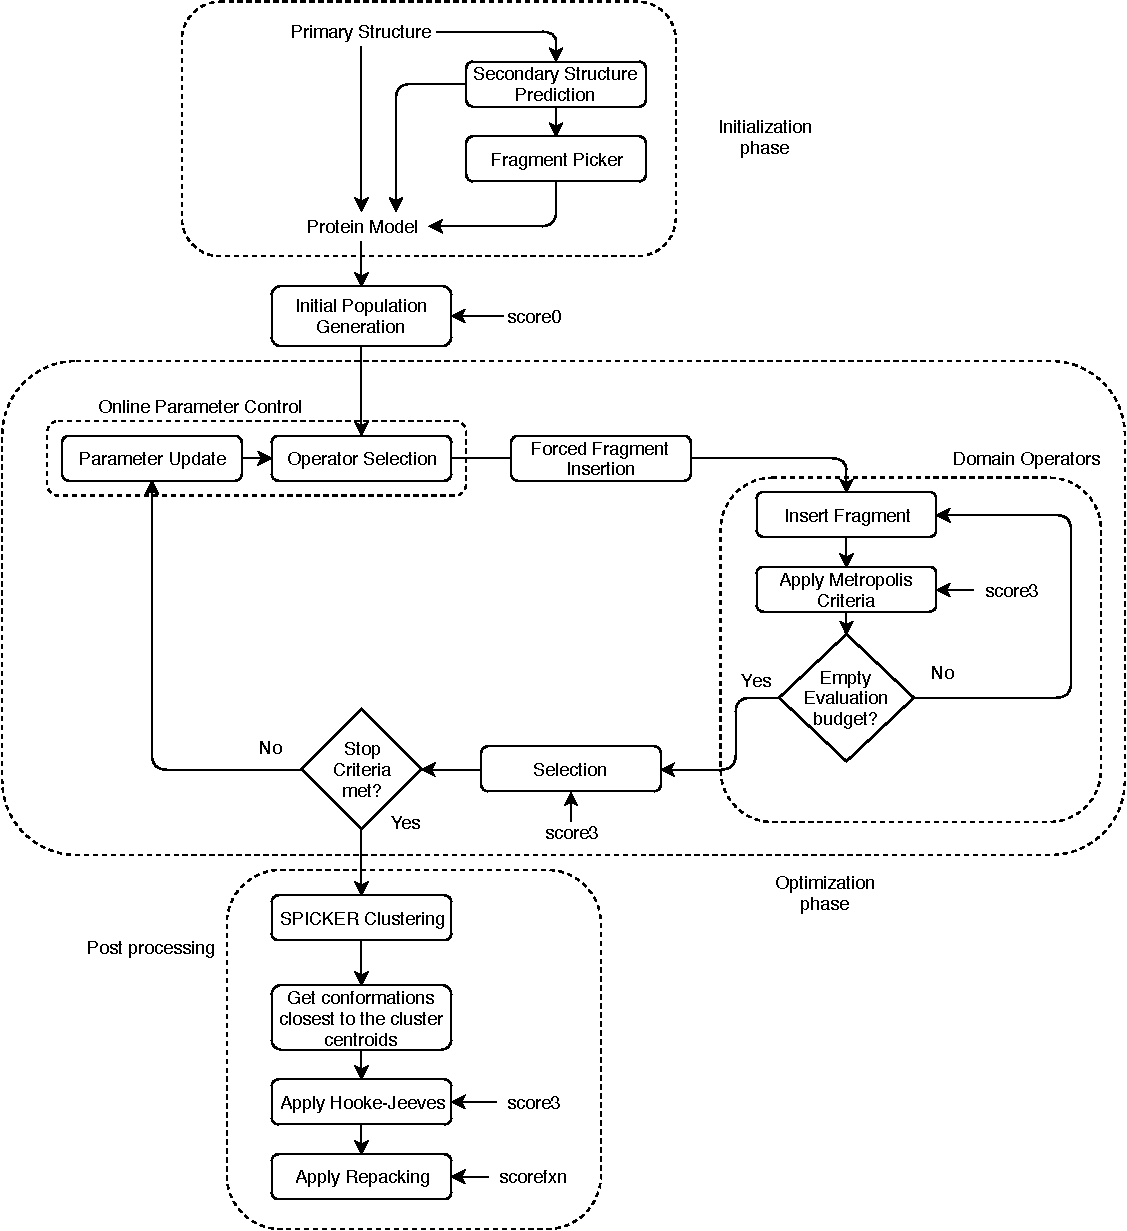
\includegraphics[width=\linewidth]{Figuras/search-procedure.pdf}
    \caption{The Proposed Search Procedure (Source: Author)}
    \label{fig:search-procedure}
\end{figure}

In the initialization phase the primary sequence is taken as input in the FASTA
format, which consists of the one letter code sequence of amino acids. The
primary sequence is then stored for later use. It is also used as input for
PSIPRED, the secondary structure predictor. PSIPRED outputs a probability
matrix mapping probabilities for the cartesian product of secondary structures
versus the amino acid sequence. This output is also stored for later use and is
fed into the fragment picker.  The fragment picker used is the Rosetta Fragment
Picker and it is responsible for selecting a set of fragments for all possible
combinations of contiguous amino acids of size 3 and 9. The fragment set is
stored to be used as input for tertiary prediction routine. Since the
initialization phase consists only of preprocessing, its time is not taken into
account when measuring the time required to predict a given target protein.
Specially considering the waiting time for the PSIPRED server.

The second phase is the optimization phase.  It starts with the step of
generating the initial population. The initial population generation consists
of assembly random protein conformations using the fragments generated in the
initialization phase. A Monte Carlo search is ran using the score0 energy
function in order to search for protein conformations that have no (or as few
as possible) hysterical clashes. This step stops when a fixed number of samples
is used for each solution vector in the population or when the score0 function
reaches zero.

With the initial population generated, the optimization procedure itself starts
guided by the score3 energy function. The basis of the search procedure is
carried out by the \ac{SaDE} algorithm, which consists of the \textit{Online
Parameter Control} part without the \textit{Differential Evolution Operators}.
The hybridization happens when the \textit{Domain Operators} are added to the
search procedure.

Firstly, the online parameter control portion of \ac{SaDE} selects which
operator to use for each individual in the population.
%
The operators can be either \ac{MC} or \ac{REMC}, with different fragment sizes.
Once it is selected, a small sub search procedure starts, corresponding to the
operator itself.
%
Before the operator is applied, the check for \ac{FFI} happens. The check occurs
for all solution vectors. If the \ac{FFI} check passes, then a random fragment
is applied. Regardless of \ac{FFI} being used or not, the next step is to apply
the standard fragment insertion.
%
A \ac{MC} or \ac{REMC} search procedure is initialized,
based on the operator chosen. This search takes a fixed amount of function
evaluation that is fed as a parameter. When this search procedure stops the
output is fed to the selection routine. From there it is checked if the stop
criteria was met. If it was not, then the parameter update routine is called,
updating the parameters F and Cr (for all operators) as well as the
probabilities for each operator. Since \ac{DE} is not used, the $Cr$ parameter
actually controller the \ac{MC} temperature parameter. The parameter control is
agnostic to which parameter it is updating. Once the Parameter Update step is
finished, the optimization cycle starts over again from the operator selection.

The when stop criteria is ultimately met, the optimization phase stops and the
post processing phase starts. The first post-processing step is to cluster the
conformations. After the clustering process finishes, the cluster centroids are
selected. The number of clusters are a parameter of the algorithm.
The conformations closest to the centroids are found and feed forward
to the next steps, while the centroids themselves are discarded. A Hooke-Jeeves
local search is applied. This helps to reach nearby local minima that might have
been inaccessible by the fragments alone. Once the local search finishes, the
repacking procedure is applied to all the conformations that were selected in
the clustering phase and then re-optimized. The repacking procedure removes the
centroids and places rotamers (side-chains fragments). The conformation is again
re-optimized, this time using a gradient descent guided by the scorefxn energy
function. After this step finishes the conformations are returned. Returning
the conformation nearest to each centroid (and re-optimizing/repacking it) allows
for a human specialist to inspect multiple conformations that are apart from
each other and select the best one. In this way, one run can provide multiple
potentially useful solutions.

Two variant of this algorithm exist. One using \ac{MC} for the fragment insertion
and the other using \ac{REMC}. It is expected that the \ac{MC} variant will have
a bigger overall diversity, and thus, returning conformations that are more
different apart. Meanwhile, the \ac{REMC} variant is expect to exploit more at
the expense of conformation diversity. That is, it may get stuck in a local
minima more easily in exchange for a increased chance of finding a better solution.
The first method is named SADE-MC-FINAL and the second is named SADE-REMC-FINAL.